\hypertarget{Types_8h}{
\section{Types.h File Reference}
\label{Types_8h}\index{Types.h@{Types.h}}
}


This graph shows which files directly or indirectly include this file:\begin{figure}[H]
\begin{center}
\leavevmode
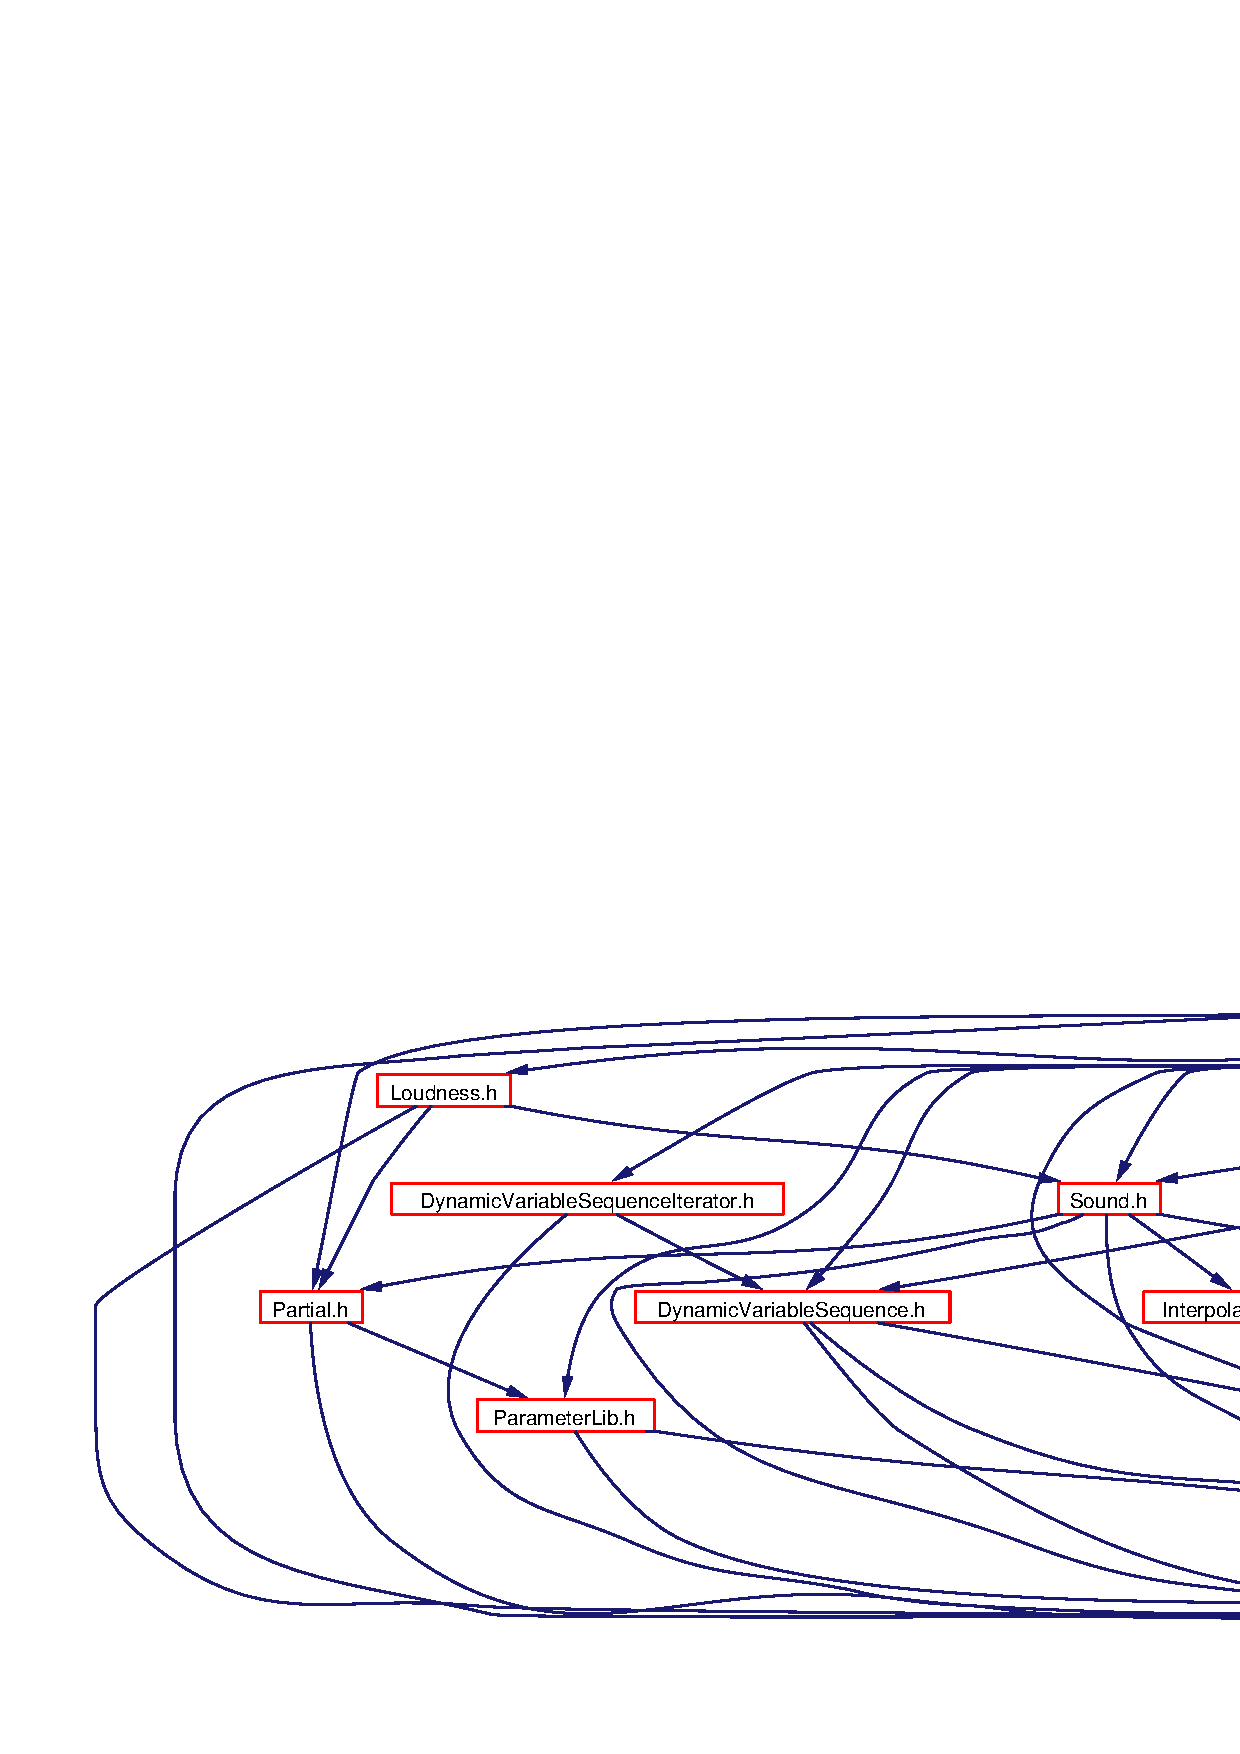
\includegraphics[width=420pt]{Types_8h__dep__incl}
\end{center}
\end{figure}
\subsection*{Classes}
\begin{CompactItemize}
\item 
struct \hyperlink{structenv__seg}{env\_\-seg}
\item 
struct \hyperlink{structenvelope__segment}{envelope\_\-segment}
\item 
struct \hyperlink{structxy__point}{xy\_\-point}
\end{CompactItemize}
\subsection*{Typedefs}
\begin{CompactItemize}
\item 
typedef float \hyperlink{Types_8h_a0}{m\_\-sample\_\-type}
\begin{CompactList}\small\item\em Specifies a type for an individual sample value. \item\end{CompactList}\item 
typedef long \hyperlink{Types_8h_a1}{m\_\-sample\_\-count\_\-type}
\begin{CompactList}\small\item\em Specifies a sample count. \item\end{CompactList}\item 
typedef float \hyperlink{Types_8h_a2}{m\_\-time\_\-type}
\begin{CompactList}\small\item\em Specifies a type for an individual time value. \item\end{CompactList}\item 
typedef float \hyperlink{Types_8h_a3}{m\_\-value\_\-type}
\begin{CompactList}\small\item\em Specifies a value type (used for frequency and amplitude). \item\end{CompactList}\item 
typedef unsigned int \hyperlink{Types_8h_a4}{m\_\-rate\_\-type}
\begin{CompactList}\small\item\em Specifies a rate for playback. \item\end{CompactList}\end{CompactItemize}
\subsection*{Enumerations}
\begin{CompactItemize}
\item 
enum \hyperlink{Types_8h_a12}{stretch\_\-type} \{ \par
\hyperlink{Types_8h_a12a7}{FIXED}, 
\par
\hyperlink{Types_8h_a12a8}{FLEXIBLE}
 \}
\item 
enum \hyperlink{Types_8h_a13}{interpolation\_\-type} \{ \par
\hyperlink{Types_8h_a13a9}{EXPONENTIAL}, 
\par
\hyperlink{Types_8h_a13a10}{CUBIC\_\-SPLINE}, 
\par
\hyperlink{Types_8h_a13a11}{LINEAR}
 \}
\end{CompactItemize}
\subsection*{Variables}
\begin{CompactItemize}
\item 
const  \hyperlink{Types_8h_a4}{m\_\-rate\_\-type} \hyperlink{Types_8h_a5}{DEFAULT\_\-SAMPLING\_\-RATE} = 44100
\begin{CompactList}\small\item\em When no sampling rate is specified, uses 44.1k\-Hz. \item\end{CompactList}\item 
const  \hyperlink{Types_8h_a4}{m\_\-rate\_\-type} \hyperlink{Types_8h_a6}{DEFAULT\_\-LOUDNESS\_\-RATE} = 10
\begin{CompactList}\small\item\em \hyperlink{classLoudness}{Loudness} can be calculated at much slower rates. The default rate is 10Hz. \item\end{CompactList}\end{CompactItemize}


\subsection{Detailed Description}
This file is included to define basic filetypes for the application. In this manner, we can easily change from float-sound to double-sound by editing one line of code. \begin{Desc}
\item[Author:]Braden Kowitz\end{Desc}


Definition in file \hyperlink{Types_8h-source}{Types.h}.

\subsection{Typedef Documentation}
\hypertarget{Types_8h_a4}{
\index{Types.h@{Types.h}!m_rate_type@{m\_\-rate\_\-type}}
\index{m_rate_type@{m\_\-rate\_\-type}!Types.h@{Types.h}}
\subsubsection[m\_\-rate\_\-type]{\setlength{\rightskip}{0pt plus 5cm}typedef unsigned int \hyperlink{Types_8h_a4}{m\_\-rate\_\-type}}}
\label{Types_8h_a4}


Specifies a rate for playback. 



Definition at line 53 of file Types.h.

Referenced by Envelope::add\-Interpolators(), Dynamic\-Variable\-Sequence::add\-Interpolators(), Loudness::calculate(), Reverb::construct\-Amp(), Reverb::Constructor\-Common(), Sound\-Sample::get\-Sampling\-Rate(), Dynamic\-Variable::get\-Sampling\-Rate(), Multi\-Track::Multi\-Track(), Sound::render(), Score::render(), Partial::render(), Reverb::Reverb(), Sound\-Sample::set\-Sampling\-Rate(), Dynamic\-Variable::set\-Sampling\-Rate(), Sound\-Sample::Sound\-Sample(), Pan::spatialize(), Multi\-Pan::spatialize(), Track::Track(), and Au\-Writer::write().\hypertarget{Types_8h_a1}{
\index{Types.h@{Types.h}!m_sample_count_type@{m\_\-sample\_\-count\_\-type}}
\index{m_sample_count_type@{m\_\-sample\_\-count\_\-type}!Types.h@{Types.h}}
\subsubsection[m\_\-sample\_\-count\_\-type]{\setlength{\rightskip}{0pt plus 5cm}typedef long \hyperlink{Types_8h_a1}{m\_\-sample\_\-count\_\-type}}}
\label{Types_8h_a1}


Specifies a sample count. 



Definition at line 44 of file Types.h.

Referenced by Score::anticlip(), Interpolator\-Iterator::append(), Loudness::calculate(), Score::channel\-Anticlip(), Score::channel\-Scale(), Score::clip(), Sound\-Sample::composite(), Constant::Constant\-Iterator::Constant\-Iterator(), Reverb::construct\-Amp(), Interpolator\-Iterator::Entry::Entry(), Sound\-Sample::get\-Sample\-Count(), Dynamic\-Variable::get\-Sample\-Count(), Multi\-Track::Multi\-Track(), Sound\-Sample::operator\mbox{[}$\,$\mbox{]}(), Sound::render(), Score::render(), Partial::render(), Score::scale(), Sound\-Sample::Sound\-Sample(), Pan::spatialize(), Multi\-Pan::spatialize(), Track::Track(), Cubic\-Spline\-Interpolator::value\-Iterator(), Exponential\-Interpolator::value\-Iterator(), Linear\-Interpolator::value\-Iterator(), and Au\-Writer::write().\hypertarget{Types_8h_a0}{
\index{Types.h@{Types.h}!m_sample_type@{m\_\-sample\_\-type}}
\index{m_sample_type@{m\_\-sample\_\-type}!Types.h@{Types.h}}
\subsubsection[m\_\-sample\_\-type]{\setlength{\rightskip}{0pt plus 5cm}typedef float \hyperlink{Types_8h_a0}{m\_\-sample\_\-type}}}
\label{Types_8h_a0}


Specifies a type for an individual sample value. 



Definition at line 41 of file Types.h.

Referenced by Score::anticlip(), Score::channel\-Scale(), Reverb::construct\-Amp(), LPComb\-Filter::do\_\-filter(), Low\-Pass\-Filter::do\_\-filter(), All\-Pass\-Filter::do\_\-filter(), Reverb::do\_\-reverb(), Sound\-Sample::operator\mbox{[}$\,$\mbox{]}(), Score::scale(), and Au\-Writer::write().\hypertarget{Types_8h_a2}{
\index{Types.h@{Types.h}!m_time_type@{m\_\-time\_\-type}}
\index{m_time_type@{m\_\-time\_\-type}!Types.h@{Types.h}}
\subsubsection[m\_\-time\_\-type]{\setlength{\rightskip}{0pt plus 5cm}typedef float \hyperlink{Types_8h_a2}{m\_\-time\_\-type}}}
\label{Types_8h_a2}


Specifies a type for an individual time value. 



Definition at line 47 of file Types.h.

Referenced by Interpolator::add\-Entry(), Dynamic\-Variable\-Sequence::add\-Interpolators(), Dynamic\-Variable\-Sequence::Add\-To\-Shape(), Interpolator\-Iterator::append(), Loudness::calculate(), Track::composite(), Sound\-Sample::composite(), Multi\-Track::composite(), Reverb::Constructor\-Common(), Interpolator\-Iterator::Entry::Entry(), Envelope::generate\-Lengths(), Dynamic\-Variable\-Sequence::generate\-Times(), Dynamic\-Variable::get\-Duration(), Dynamic\-Variable\-Sequence::get\-Segment\-Time(), Sound::get\-Total\-Duration(), Partial::get\-Total\-Duration(), Dynamic\-Variable\-Sequence::get\-Value(), Interpolator\-Entry::Interpolator\-Entry(), Envelope\-Library::load\-Library(), Cubic\-Spline\-Interpolator\-Iterator::next(), Exponential\-Interpolator\-Iterator::next(), Sound::render(), Score::render(), Partial::render(), Dynamic\-Variable::set\-Duration(), Dynamic\-Variable\-Sequence::set\-Segment\-Time(), Cubic\-Spline\-Interpolator::value\-Iterator(), Exponential\-Interpolator::value\-Iterator(), Linear\-Interpolator::value\-Iterator(), and Au\-Writer::write().\hypertarget{Types_8h_a3}{
\index{Types.h@{Types.h}!m_value_type@{m\_\-value\_\-type}}
\index{m_value_type@{m\_\-value\_\-type}!Types.h@{Types.h}}
\subsubsection[m\_\-value\_\-type]{\setlength{\rightskip}{0pt plus 5cm}typedef float \hyperlink{Types_8h_a3}{m\_\-value\_\-type}}}
\label{Types_8h_a3}


Specifies a value type (used for frequency and amplitude). 



Definition at line 50 of file Types.h.

Referenced by Interpolator::add\-Entry(), Envelope::add\-Interpolators(), Envelope::Add\-To\-Shape(), Interpolator\-Iterator::append(), Loudness::calculate(), Constant::Constant(), Constant::Constant\-Iterator::Constant\-Iterator(), Loudness::critical\-Band\-Index(), Envelope::Define\-Shape(), Interpolator\-Iterator::Entry::Entry(), Loudness::Critical\-Band::get\-Band\-Gamma(), Interpolator::get\-Max\-Value(), Envelope::get\-Max\-Value(), Dynamic\-Variable\-Sequence::get\-Max\-Value(), Constant::get\-Max\-Value(), Loudness::Partial\-Snapshot::get\-Scaling\-Factor(), Envelope::get\-Segment\-Length(), Envelope::get\-Value(), Dynamic\-Variable\-Sequence::get\-Value(), Constant::get\-Value(), Interpolator\-Entry::Interpolator\-Entry(), Cubic\-Spline\-Interpolator\-Iterator::next(), Exponential\-Interpolator\-Iterator::next(), Linear\-Interpolator\-Iterator::next(), Envelope\-Iterator::next(), Dynamic\-Variable\-Sequence\-Iterator::next(), Loudness::Partial\-Snapshot::Partial\-Snapshot(), Partial::pmod(), Partial::render(), Track::scale(), Sound\-Sample::scale(), Interpolator::scale(), Envelope::scale(), Dynamic\-Variable\-Sequence::scale(), Constant::scale(), Parameter\-Lib$<$ Static\-T, Dynamic\-T $>$::set\-Param(), Sound::set\-Partial\-Param(), Envelope::set\-Segment\-Length(), Constant::set\-Value(), Sound::Sound(), Pan::spatialize(), Multi\-Pan::spatialize(), Cubic\-Spline\-Interpolator::value\-Iterator(), Exponential\-Interpolator::value\-Iterator(), and Linear\-Interpolator::value\-Iterator().

\subsection{Enumeration Type Documentation}
\hypertarget{Types_8h_a13}{
\index{Types.h@{Types.h}!interpolation_type@{interpolation\_\-type}}
\index{interpolation_type@{interpolation\_\-type}!Types.h@{Types.h}}
\subsubsection[interpolation\_\-type]{\setlength{\rightskip}{0pt plus 5cm}enum \hyperlink{Types_8h_a13}{interpolation\_\-type}}}
\label{Types_8h_a13}


This is used in Envelope\-Entry to specify what kind of interpolation the entry should have. \begin{Desc}
\item[Enumeration values: ]\par
\begin{description}
\index{EXPONENTIAL@{EXPONENTIAL}!Types.h@{Types.h}}\index{Types.h@{Types.h}!EXPONENTIAL@{EXPONENTIAL}}\item[{\em 
\hypertarget{Types_8h_a13a9}{
EXPONENTIAL}
\label{Types_8h_a13a9}
}]\index{CUBIC_SPLINE@{CUBIC\_\-SPLINE}!Types.h@{Types.h}}\index{Types.h@{Types.h}!CUBIC_SPLINE@{CUBIC\_\-SPLINE}}\item[{\em 
\hypertarget{Types_8h_a13a10}{
CUBIC\_\-SPLINE}
\label{Types_8h_a13a10}
}]\index{LINEAR@{LINEAR}!Types.h@{Types.h}}\index{Types.h@{Types.h}!LINEAR@{LINEAR}}\item[{\em 
\hypertarget{Types_8h_a13a11}{
LINEAR}
\label{Types_8h_a13a11}
}]\end{description}
\end{Desc}



Definition at line 66 of file Types.h.

Referenced by Cubic\-Spline\-Interpolator::get\-Type(), Exponential\-Interpolator::get\-Type(), Linear\-Interpolator::get\-Type(), Envelope\-Library::load\-Library(), Envelope::set\-Segment\-Interpolation\-Type(), and Dynamic\-Variable\-Sequence::set\-Segment\-Interpolation\-Type().\hypertarget{Types_8h_a12}{
\index{Types.h@{Types.h}!stretch_type@{stretch\_\-type}}
\index{stretch_type@{stretch\_\-type}!Types.h@{Types.h}}
\subsubsection[stretch\_\-type]{\setlength{\rightskip}{0pt plus 5cm}enum \hyperlink{Types_8h_a12}{stretch\_\-type}}}
\label{Types_8h_a12}


This is used in Envelope\-Entry to specify whether the entry should be played for a fixed amount of time or a percentage of total time. \begin{Desc}
\item[Enumeration values: ]\par
\begin{description}
\index{FIXED@{FIXED}!Types.h@{Types.h}}\index{Types.h@{Types.h}!FIXED@{FIXED}}\item[{\em 
\hypertarget{Types_8h_a12a7}{
FIXED}
\label{Types_8h_a12a7}
}]\index{FLEXIBLE@{FLEXIBLE}!Types.h@{Types.h}}\index{Types.h@{Types.h}!FLEXIBLE@{FLEXIBLE}}\item[{\em 
\hypertarget{Types_8h_a12a8}{
FLEXIBLE}
\label{Types_8h_a12a8}
}]\end{description}
\end{Desc}



Definition at line 59 of file Types.h.

Referenced by Envelope::get\-Segment\-Length\-Type(), Dynamic\-Variable\-Sequence::get\-Segment\-Time\-Type(), and Envelope\-Library::load\-Library().

\subsection{Variable Documentation}
\hypertarget{Types_8h_a6}{
\index{Types.h@{Types.h}!DEFAULT_LOUDNESS_RATE@{DEFAULT\_\-LOUDNESS\_\-RATE}}
\index{DEFAULT_LOUDNESS_RATE@{DEFAULT\_\-LOUDNESS\_\-RATE}!Types.h@{Types.h}}
\subsubsection[DEFAULT\_\-LOUDNESS\_\-RATE]{\setlength{\rightskip}{0pt plus 5cm}const \hyperlink{Types_8h_a4}{m\_\-rate\_\-type} \hyperlink{Types_8h_a6}{DEFAULT\_\-LOUDNESS\_\-RATE} = 10\hspace{0.3cm}{\tt  \mbox{[}static\mbox{]}}}}
\label{Types_8h_a6}


\hyperlink{classLoudness}{Loudness} can be calculated at much slower rates. The default rate is 10Hz. 



Definition at line 124 of file Types.h.\hypertarget{Types_8h_a5}{
\index{Types.h@{Types.h}!DEFAULT_SAMPLING_RATE@{DEFAULT\_\-SAMPLING\_\-RATE}}
\index{DEFAULT_SAMPLING_RATE@{DEFAULT\_\-SAMPLING\_\-RATE}!Types.h@{Types.h}}
\subsubsection[DEFAULT\_\-SAMPLING\_\-RATE]{\setlength{\rightskip}{0pt plus 5cm}const \hyperlink{Types_8h_a4}{m\_\-rate\_\-type} \hyperlink{Types_8h_a5}{DEFAULT\_\-SAMPLING\_\-RATE} = 44100\hspace{0.3cm}{\tt  \mbox{[}static\mbox{]}}}}
\label{Types_8h_a5}


When no sampling rate is specified, uses 44.1k\-Hz. 



Definition at line 121 of file Types.h.